\subsubsection{Front}
Un peu plus intéressant que l'opérateur S, l'opérateur front, abrégé {\em F} dans Taggre, va limiter le nombre de tâches disponibles au même moment dans l'ordonnanceur.
%
Pour cela, il va travailler à diminuer la largeur du graphe.
%
Certaines propriétés du graphe peuvent être corrélées aux résultats de l'ordonnanceur.
%
Par exemple, la hauteur d'un graphe correspondra au temps minimum qu'il faudra pour traiter tout le graphe si nous avons un nombre infini d'unité de calcul.
%
La largeur du graphe donnera un indice sur le parallélisme exploitable.
%
Plus un graphe est large, plus il offrira de parallélisme.
%
En effet, avec un nombre illimité de coeurs de calcul, on peut exploiter au mieux le même nombre de coeurs que la largeur du graphe.
%
Le cas idéal serait donc un graphe de hauteur proche de 1 avec un nombre conséquent de tâches à la même hauteur.
%
Ce cas ressemble fortement au parallélisme de boucle.
%
Le nombre de tâches du graphe est aussi une propriété à prendre en compte, l'ordonnanceur doit avoir des structures de données efficaces capables de stocker toutes les tâches.



Un graphe fournissant énormément de parallélisme par rapport au nombre de coeurs disponibles n'aura pas forcément un meilleur équilibrage de charge par rapport à un graphe offrant moins de parallélisme.
%
D'autre part, trop de parallélisme peut conduire à la congestion des structures de données servant à maintenir à jour les tâches prêtes à être ordonnancées.
%
En réduisant la largeur du graphe, on peut ainsi réduire le parallélisme.
%
Mais il faut faire attention à ne pas trop le réduire.
%
C'est pourquoi l'opérateur F prend en paramètre la largeur du graphe souhaitée.
%
L'algorithme de l'opérateur F consiste à faire un parcourt du graphe en hauteur et à limiter le nombre de tâches par hauteur, cette limite est donnée en paramètre par le programmeur (Algo.~\ref{algo:algo_F}).
%
Les tâches agrégées ensemble ont la même hauteur, il ne peut donc pas exister de chemin entre elles, il n'y a donc aucun risque de création de cycle (Fig.~\ref{fig:algo_F2}).


%   (-_-)   %
\begin{figure}[t!]
  \centering
  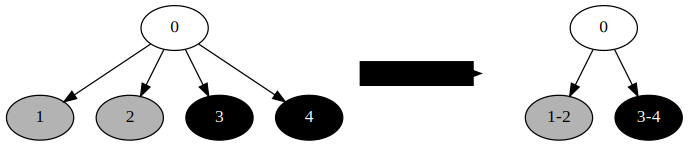
\includegraphics[width=0.7\textwidth]{algo_F2}
  \caption{Exemple d'agrégation avec l'opérateur F et le paramètre 2.}
  \label{fig:algo_F2}
\end{figure}

\begin{algorithm}
  \KwData{$MAX$, DAG}
  {\sc Suivant} = liste vide \\
  mettre les tâches racines de DAG dans {\sc Suivant} \\
  \While{{\sc Suivant} n'est pas vide} {
    {\sc Prêt} = {\sc Suivant} \\
    {\sc Suivant} = liste vide \\
    {\sc Moyenne} = taille de {\sc Prêt} / $MAX$ \\

    \While{{\sc Prêt} n'est pas vide} {
      mettre les successeurs des {\sc Moyenne} premières tâches dans {\sc Suivant} \\
      {\sc T1} = retirer le premier de {\sc Prêt} \\
      \For{{\sc $i$} allant de 0 à {\sc Moyenne}} {
        {\sc T2} = retirer le premier de {\sc Prêt} \\
        {\sc T1} devient {\sc T1} union {\sc T2}
      }
    }
  }
  \caption{Algorithme de l'opérateur front.}
  \label{algo:algo_F}
\end{algorithm}
